\subsection{Training on both GENIE and GiBUU Data}

\noindent A model was trained on both the GENIE and GiBUU datasets, and contained 61,804 samples for training, 8,830 for validation and 17,658 for testing with an equal number of the 3 interaction types, and an equal number of GENIE and GiBUU generated events.\medskip

\begin{figure}[t!]
 \centering
 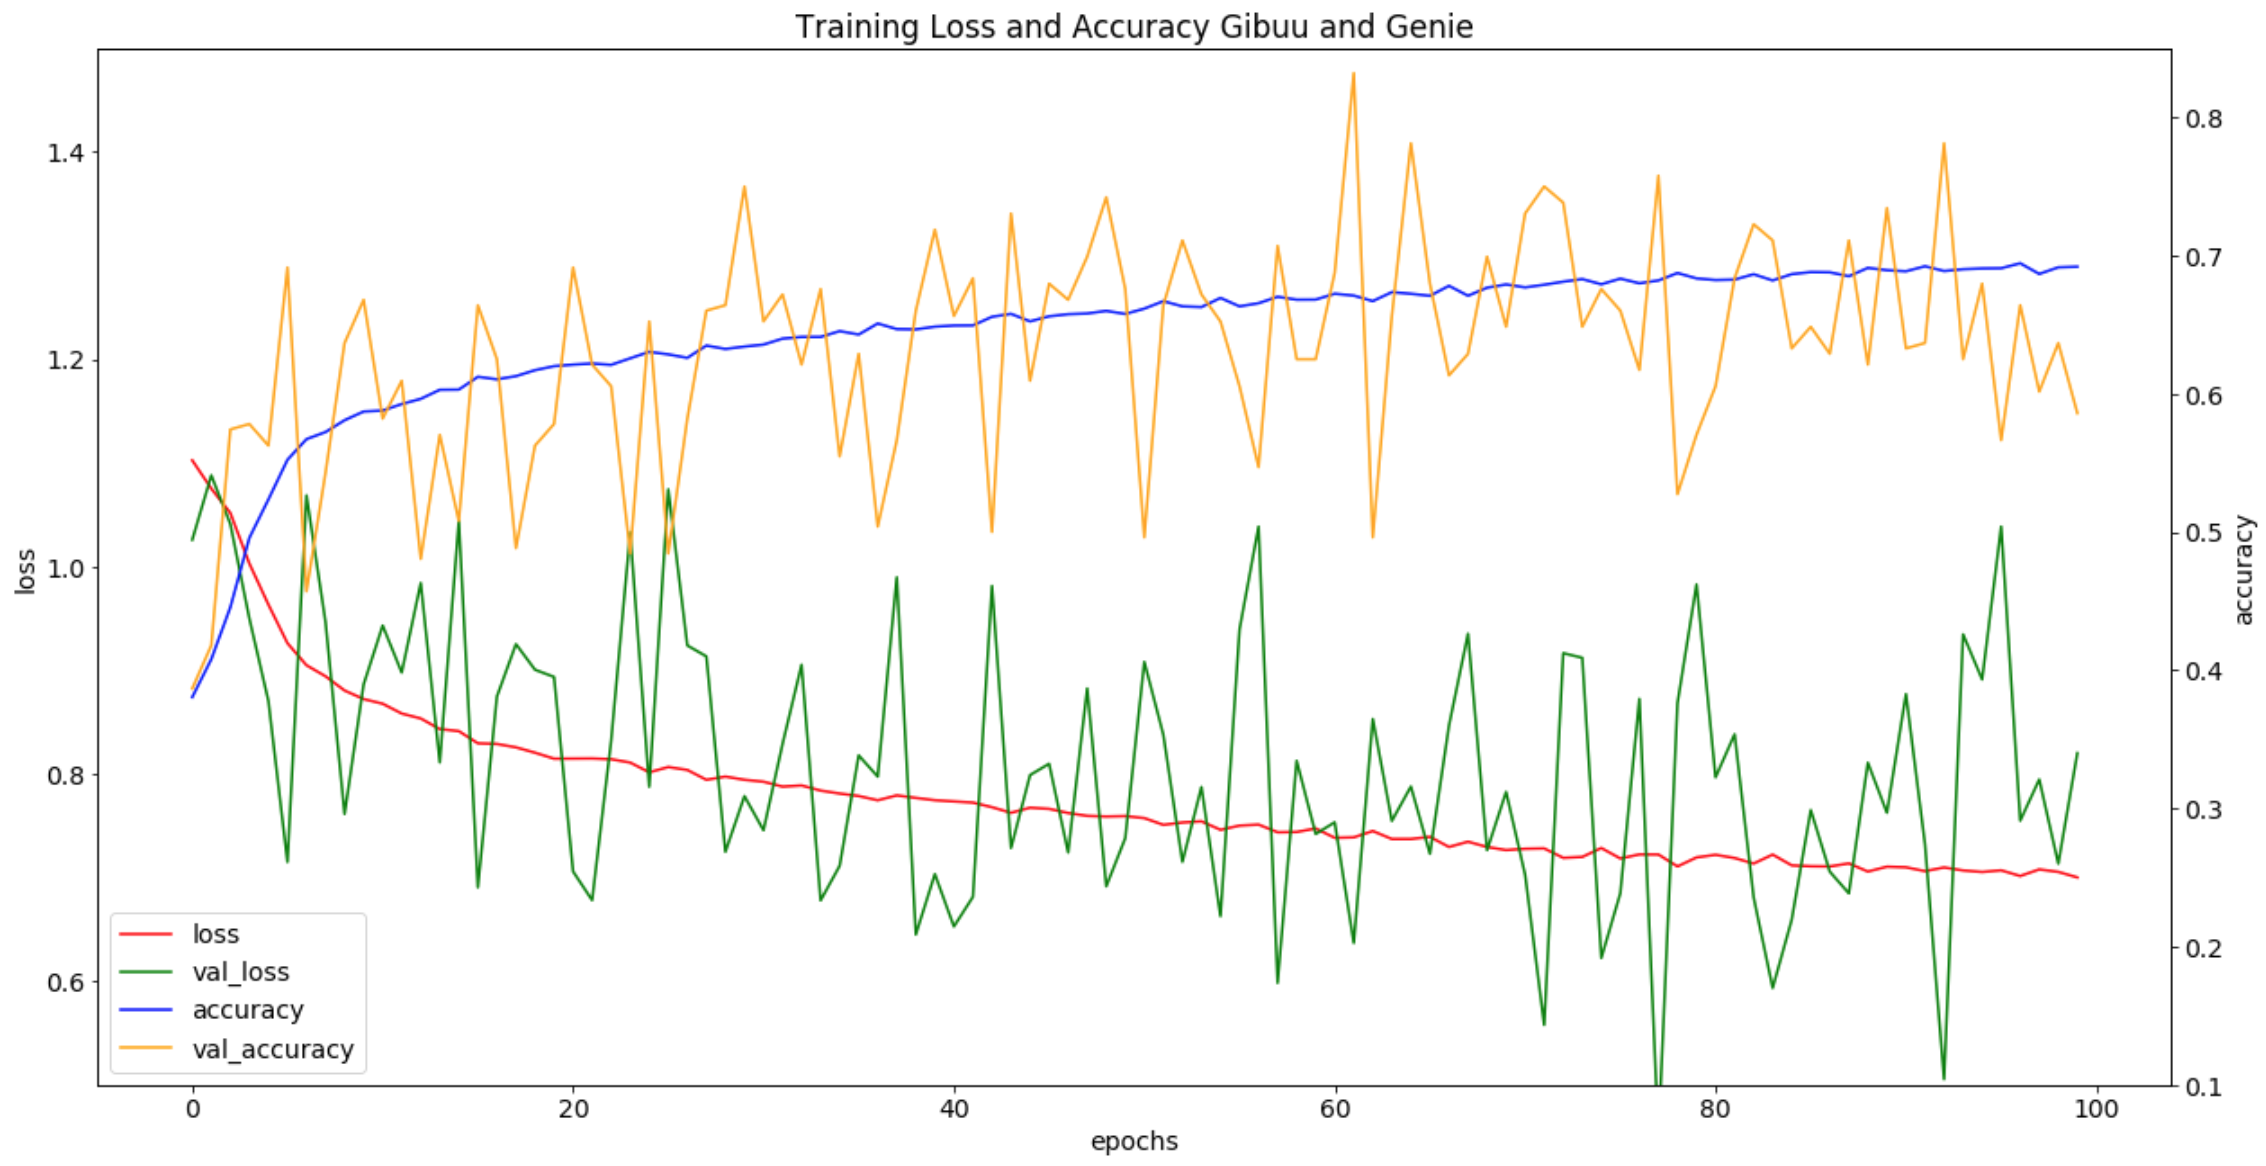
\includegraphics[width=160mm]{Both_Data/train.png}
 \textbf{Figure 21.} \textit{Network training and validation accuracy and loss.The network was trained over 100 epochs using both GENIE and GENIE generated events. With an equal number of all three event types. }
\end{figure}

\noindent From the training statistics in Figure 21, we can see that the model does not over fit the same way the imbalanced dataset did. The validation set often performs better than the training process, and this is because during the training process the dropout function is applied, so that network is classifying based on only a subset of its architecture. When then validating, all the nodes in the model are now available producing a more powerful classifier. The validation set also performs more poorly than the testing set during some epochs of the process, and this is because the network has over fit to the data it has seen and does not generalise as well to the unseen data. Overtime these two processes oscillate, however the overall trend of performance is increasing, as is expected.\medskip

\noindent Looking at the $\nu_\mu$ classifier output, Figure 22, we can see that the network performs well- better than the classifier that was trained on only GENIE events. The $\nu_\mu$ classifier successfully classifies a large proportion of the truth $\nu_\mu$ events correctly with a confidence of 90\%, while successfully classifying nearly all of the truth NC events as not $\nu_\mu$ with a confidence level of 60\% and $\nu_e$ with a confidence of 80\%. A number of truth $\nu_\mu$ events are predicted as not $\nu_\mu$ with a similar probability as the NC events, and this may be cause they are the subset of the $\nu_\mu$ that appear most similar to NC events, this will be looked into further in the Domain Classification section.\medskip

\begin{figure}[t!]
 \centering
 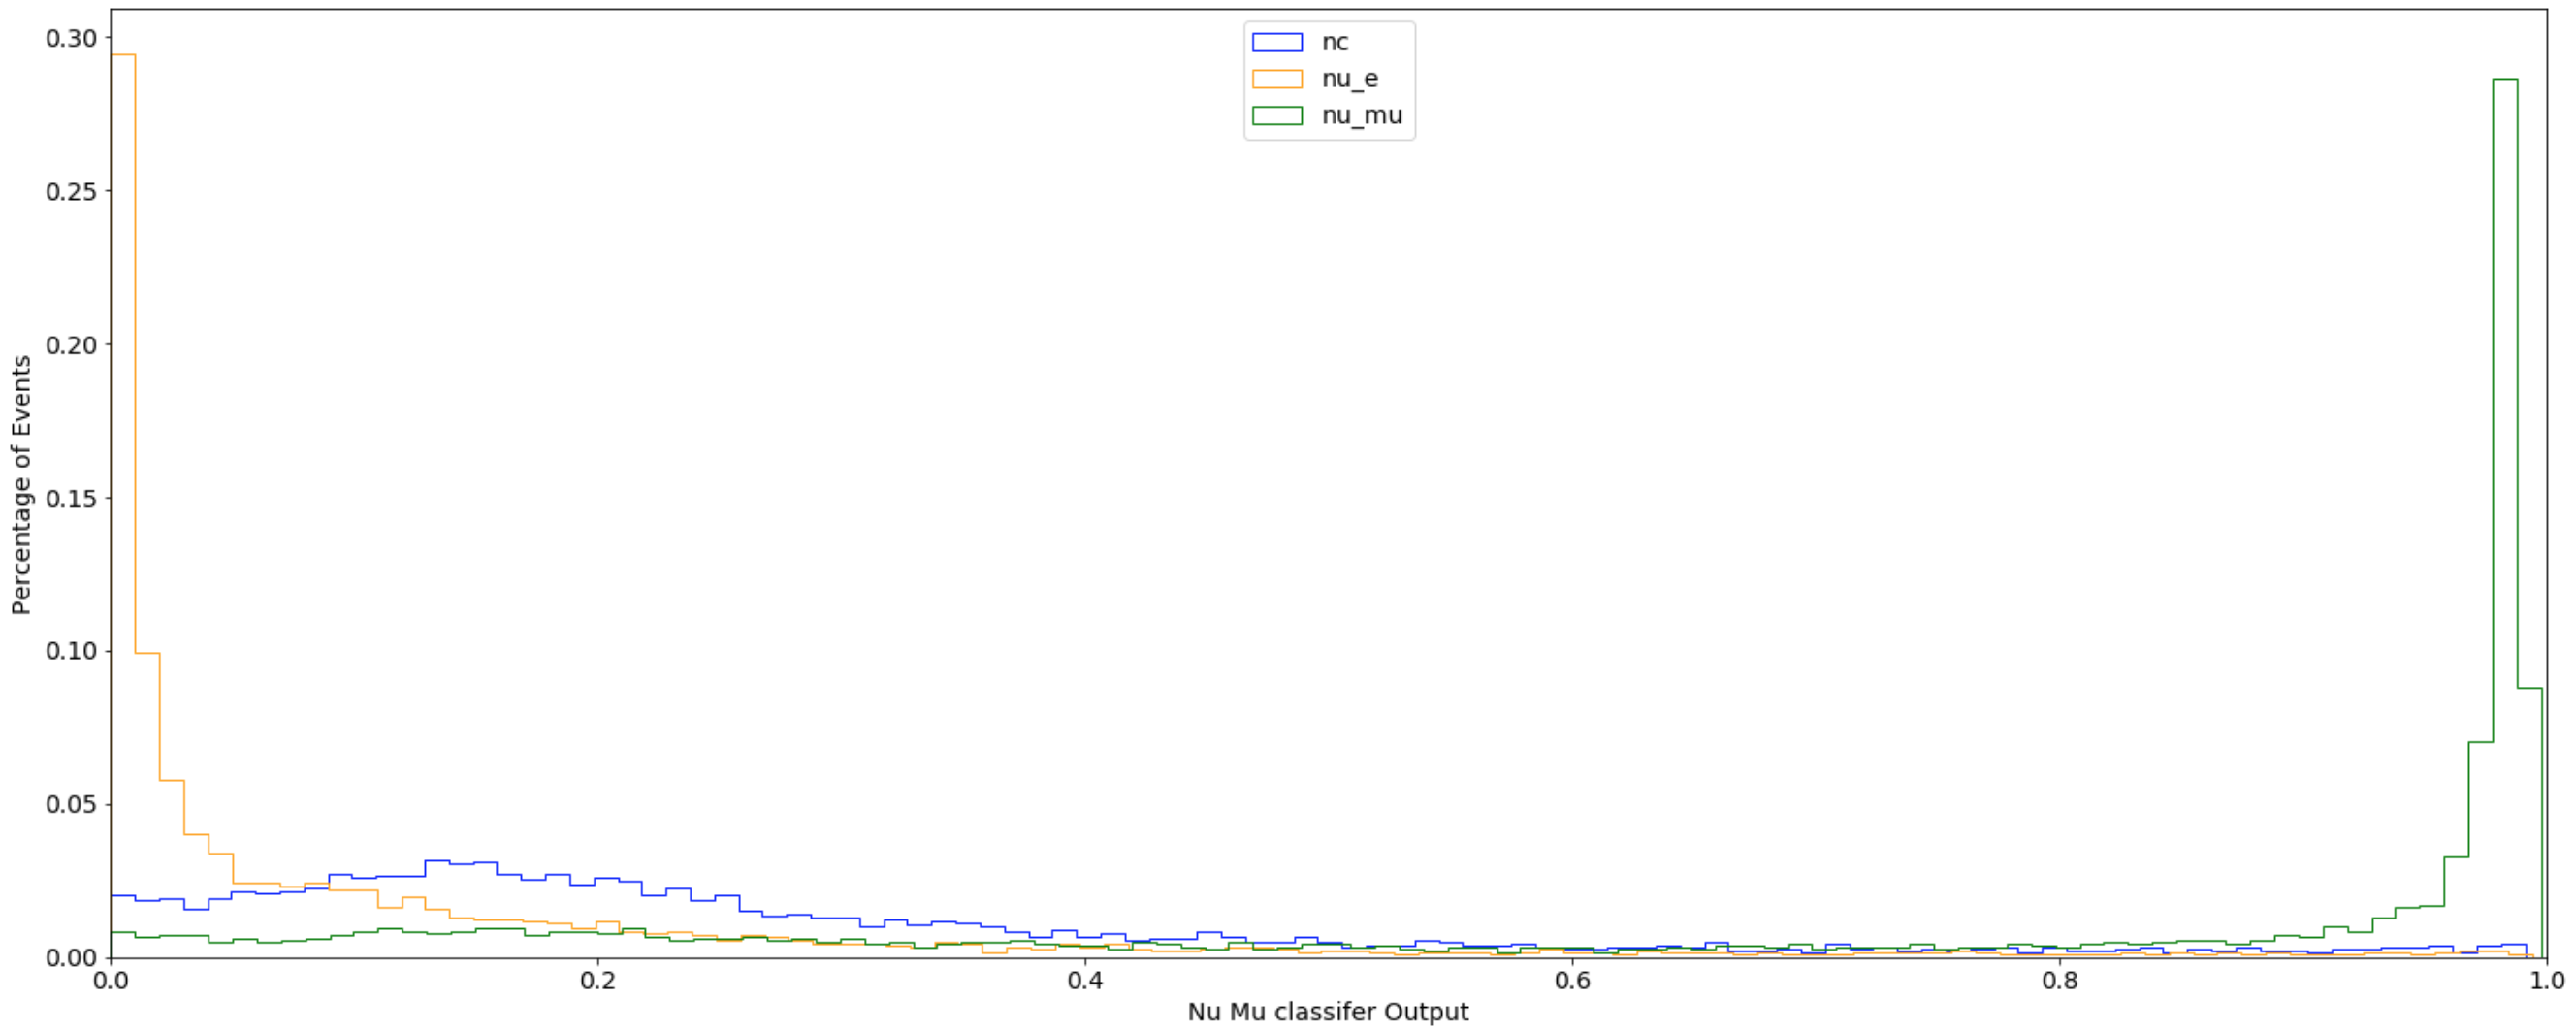
\includegraphics[width=160mm]{Both_Data/NUMU.png}
 \textbf{Figure 22.} \textit{$\nu_\mu$ classification output histogram. The dataset was trained and tested using data from both GENIE and GIBUU generated events. The dataset contained an equal number of all three event types.}

 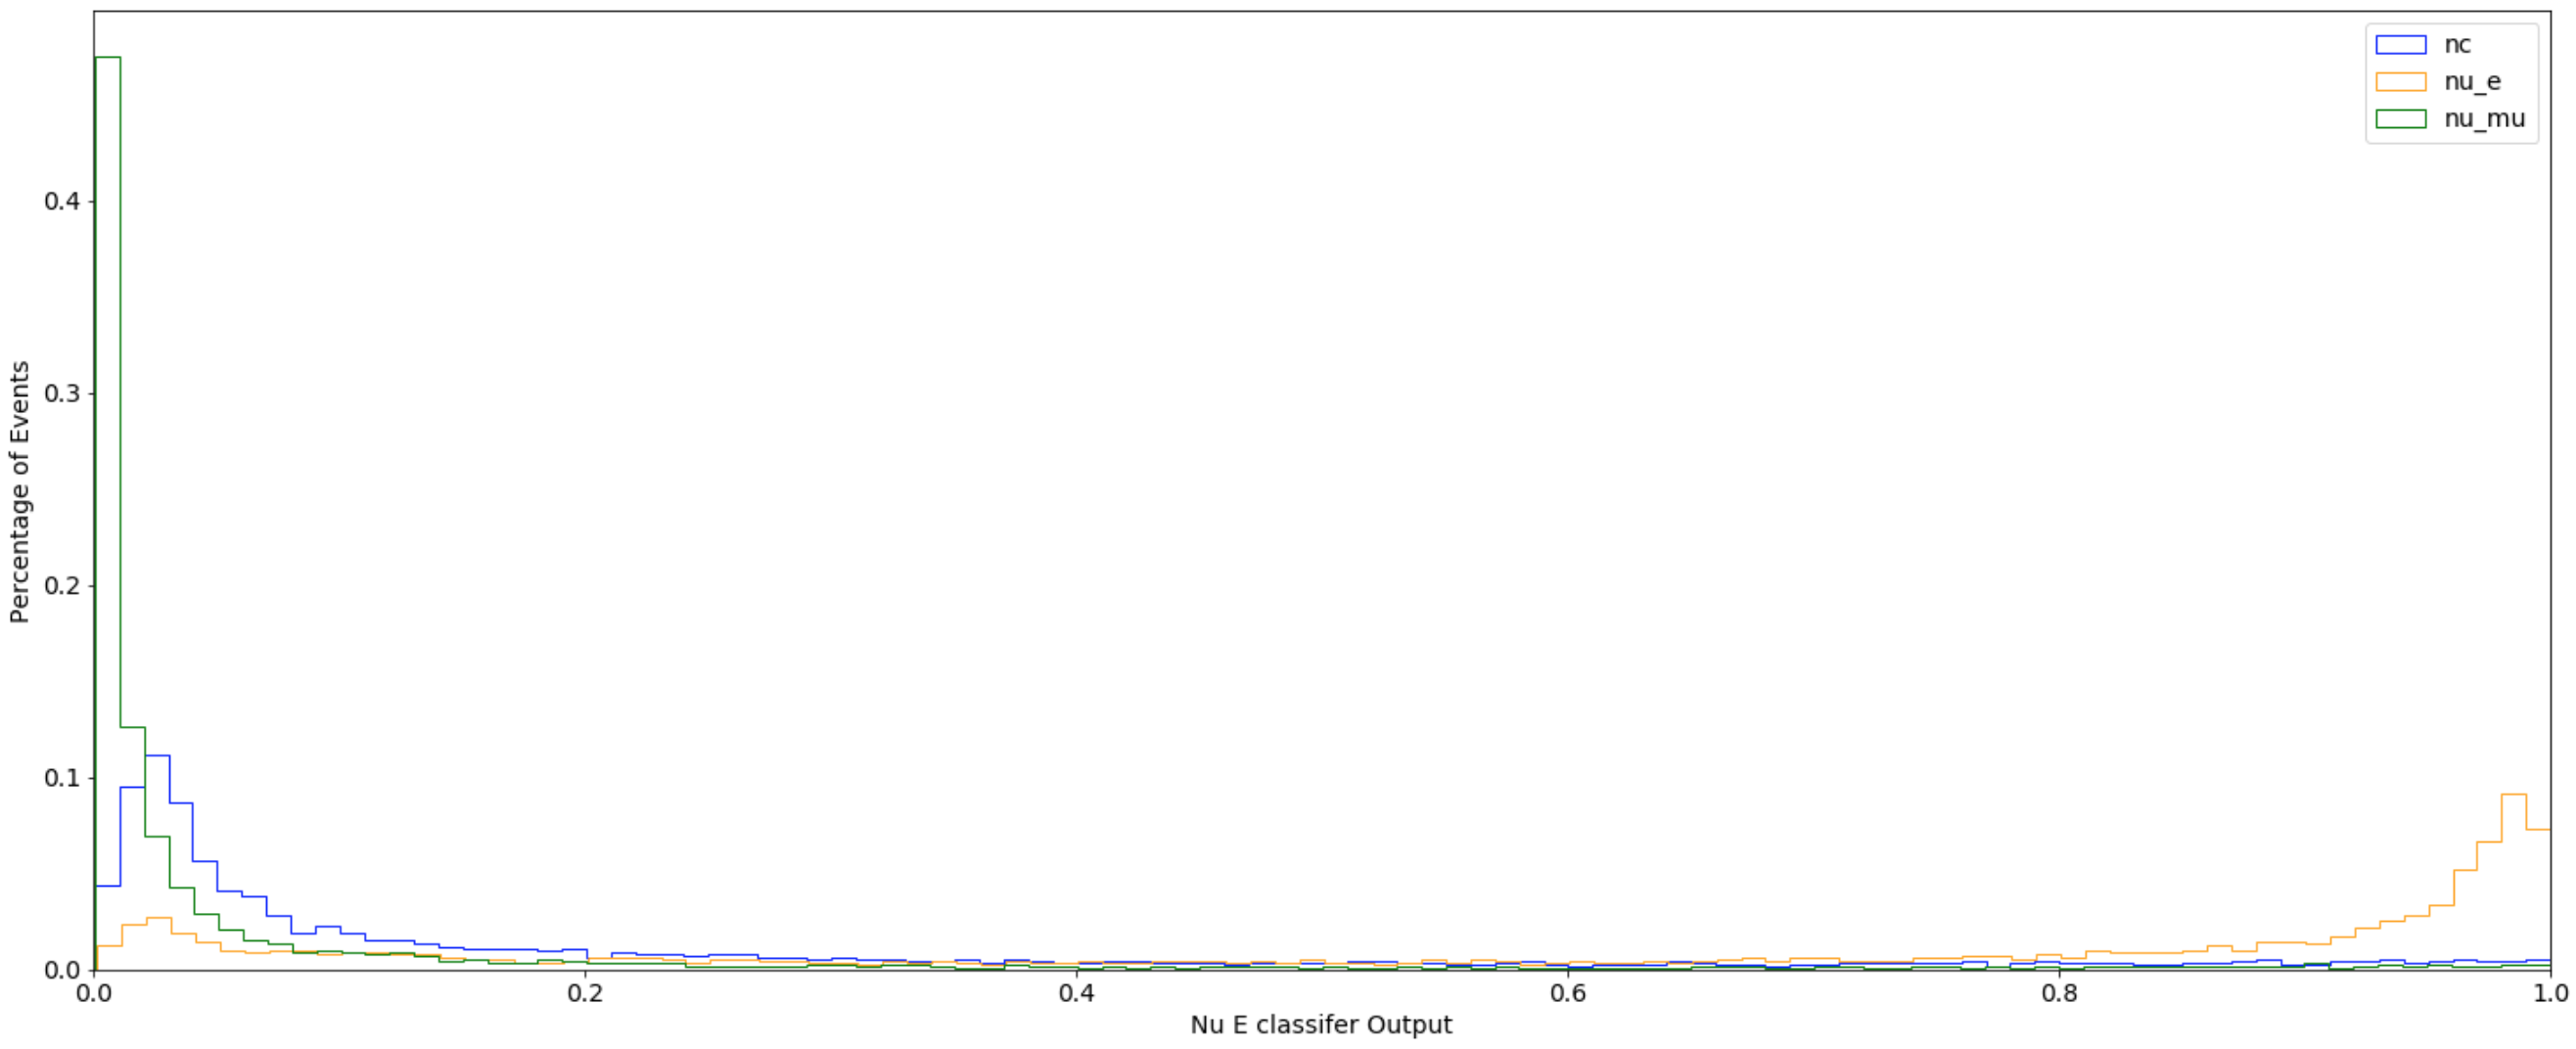
\includegraphics[width=160mm]{Both_Data/NUE.png}
 \textbf{Figure 23.} \textit{$\nu_e$ classification output histogram. The results were produced from the same training and testing process as Figures 21 and 22.}
\end{figure}

\noindent The $\nu_e$ classifier, in Figure 23, does not perform as strongly as the $\nu_\mu$ classifier, with a much smaller proprtion being correctly identified as $\nu_e$ events with a confidence of 80\%. What the $\nu_e$ does well is that it is able to correctly identify events as not $\nu_e$ events, with a large proportion of the $\nu_\mu$ and $NC$ events being classified as not $\nu_e$ events with a confidence level of 90\%. What also can be seen is again a number of $\nu_e$ are incorrectly identified as not $\nu_e$ with a similar confidence distribution as the $NC$ events, and this may be as these are the $\nu_e$ events that look similar to the $NC$ events that have large showers. \medskip

\begin{figure}[t!]
 \centering
 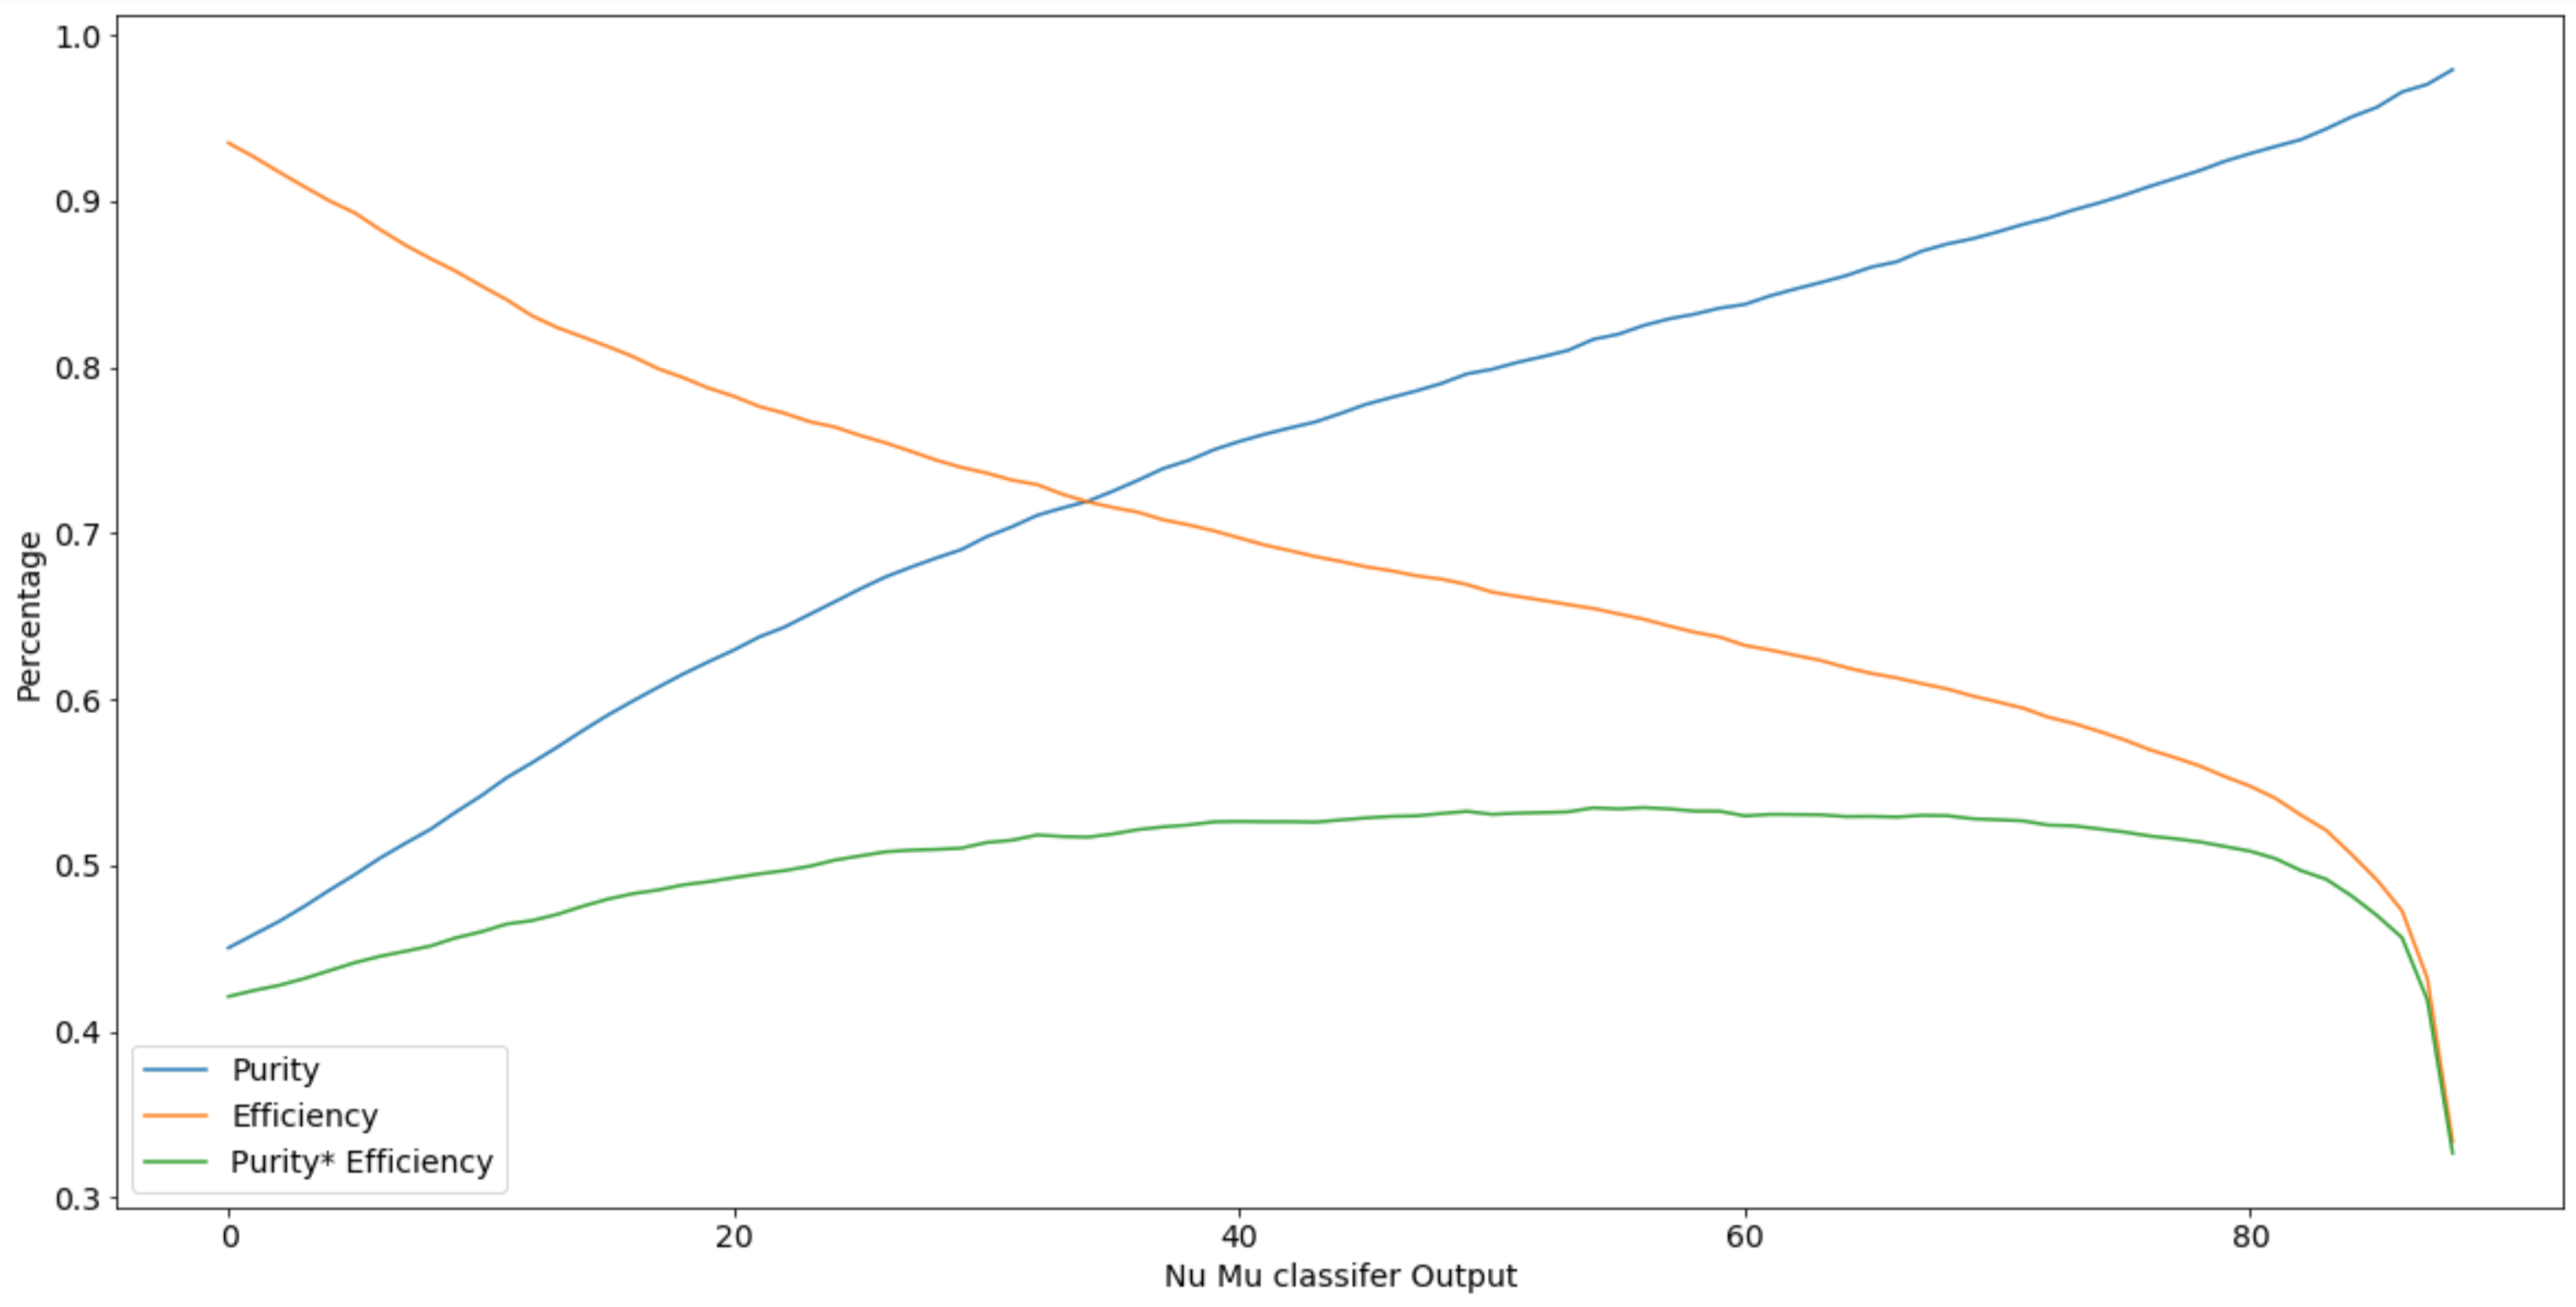
\includegraphics[width=160mm]{Both_Data/NUMUCL.png}
 \textbf{Figure 24.} \textit{$\nu_\mu$ classification output purity, efficiency and their product. The results were produced from the same training and testing process as Figures 22 and 23.}
 
 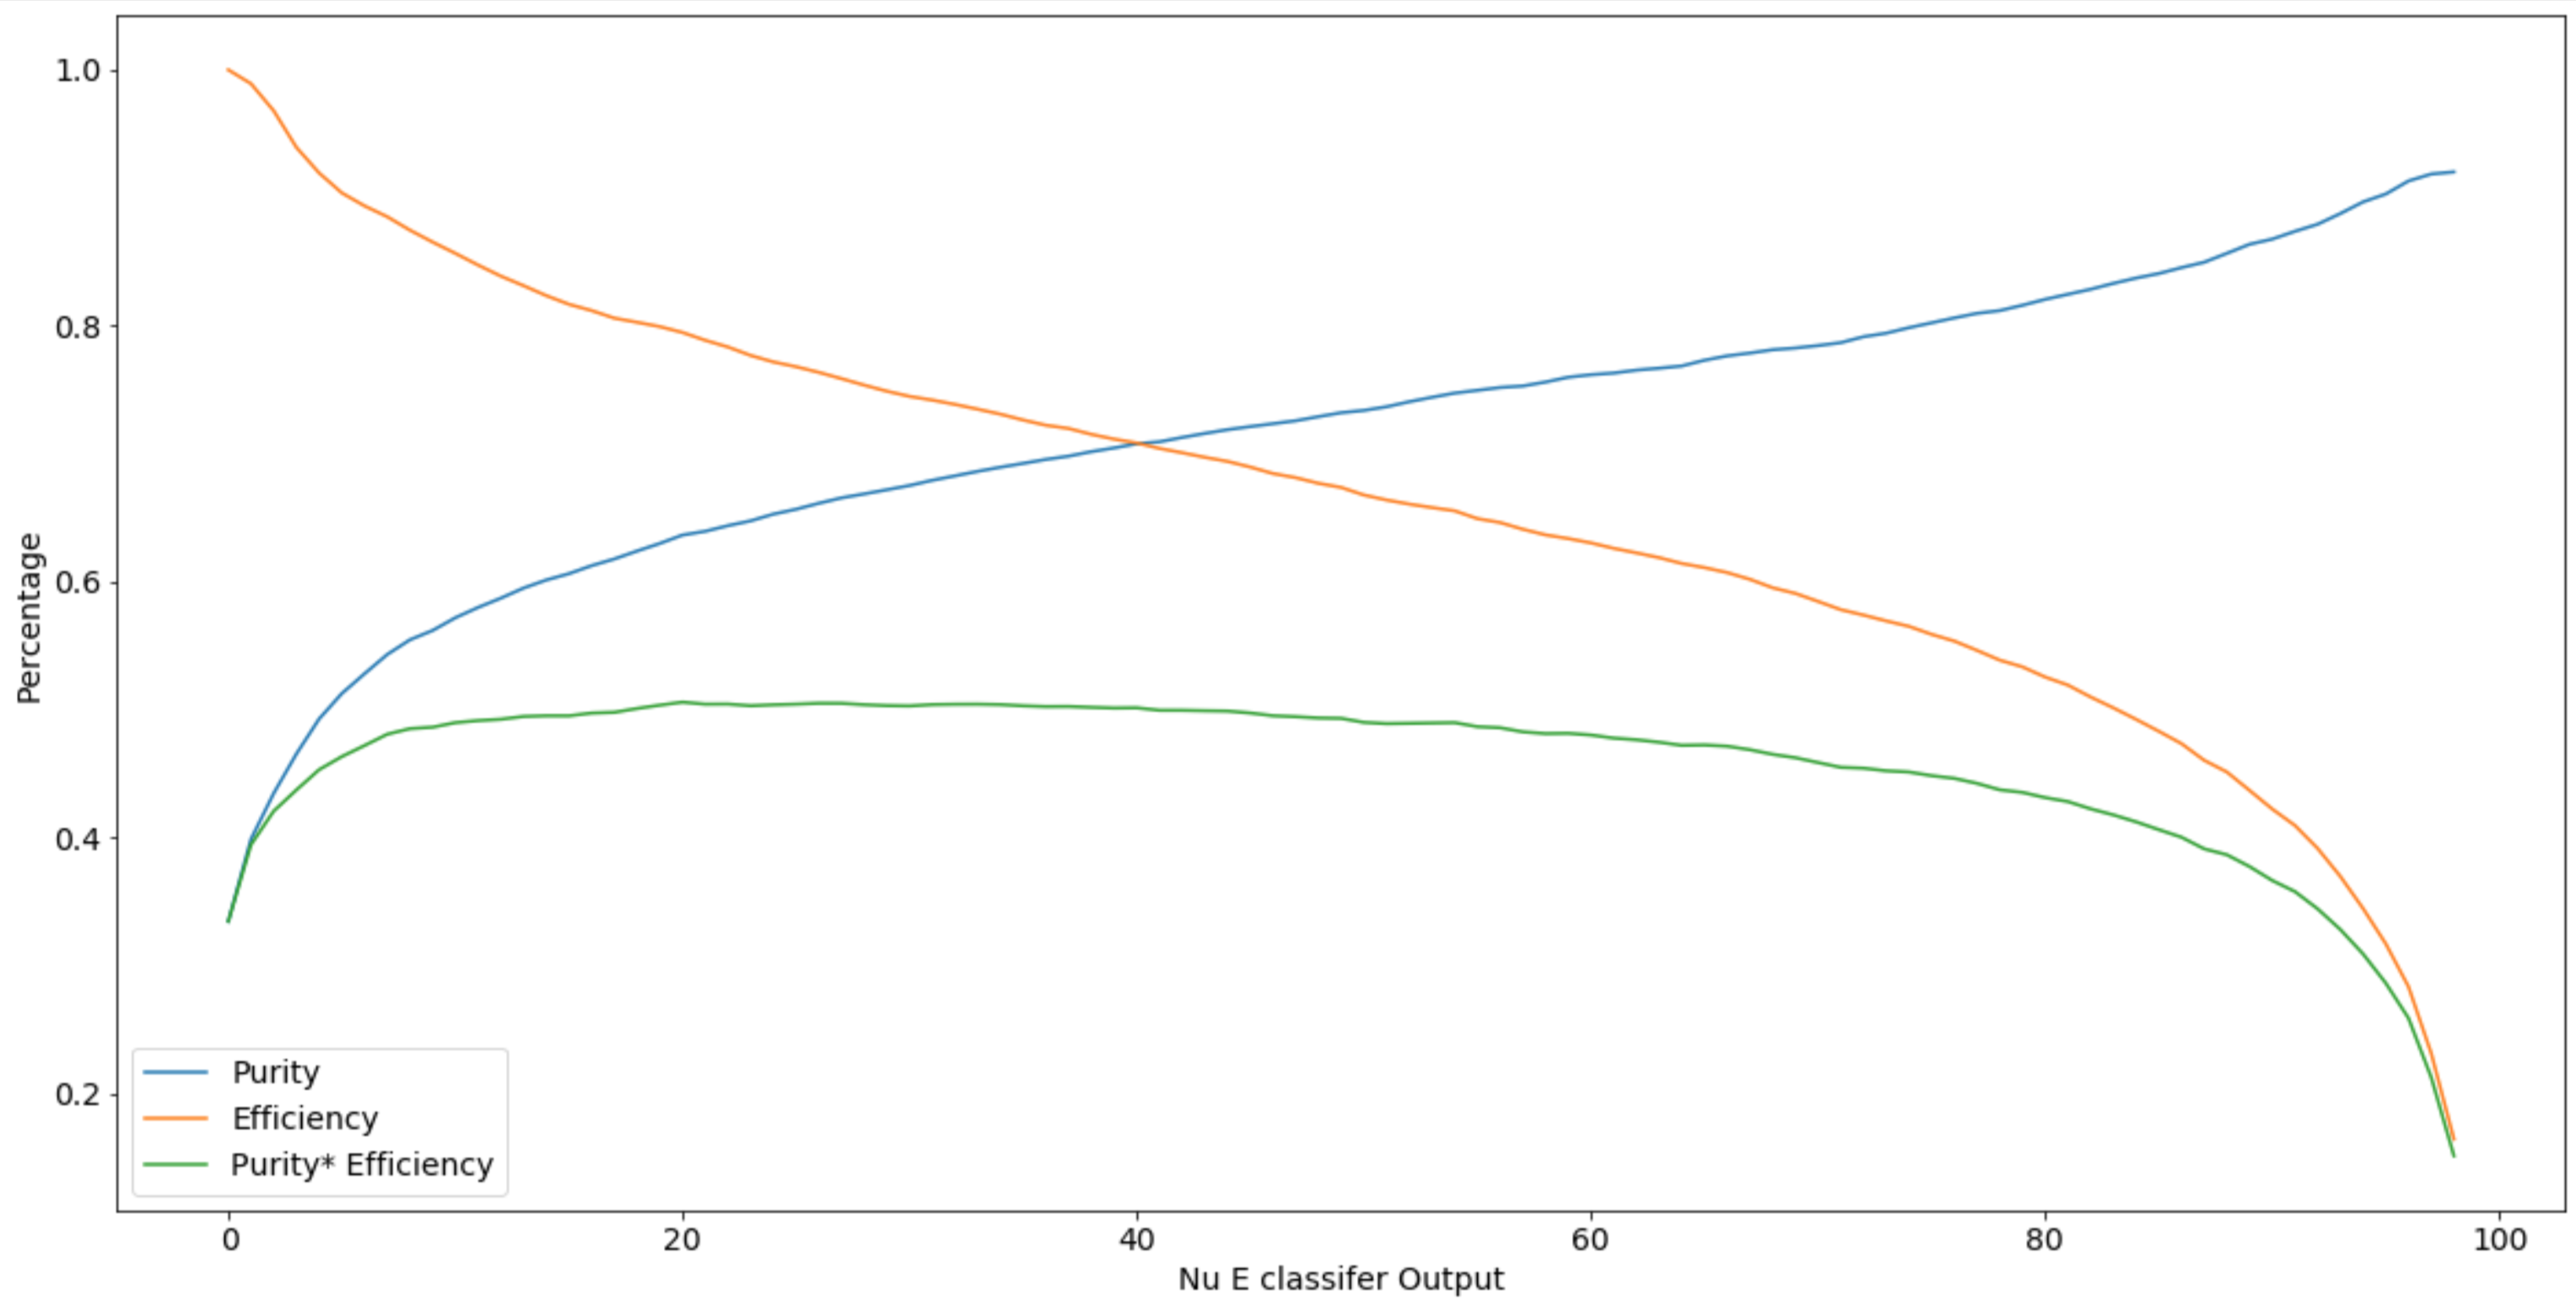
\includegraphics[width=160mm]{Both_Data/NUECL.png}
 \textbf{Figure 25.} \textit{$\nu_e$ classification output purity, efficiency and their product. The results were produced from the same training and testing process as Figures 22 and 23.}
\end{figure}


\noindent By looking at the $\nu_\mu$ purity-efficacy plot in Figure 24 and $\nu_e$ plot in Figure 25, it can be seen that the $\nu_\mu$ purity-efficiency product curve confirms the better performance that was indicated in Figure 22. The selection cut for the $\nu_\mu$ classifier would be made at a might higher value than with the $\nu_e$ classifier, and a cut at a 60\% confidence value would provide a classification accuracy, given by the purity value of 82\% while retaining 62\% of the $\nu_\mu$ events. \medskip

\begin{figure}[t!]
 \begin{subfigure}{}
 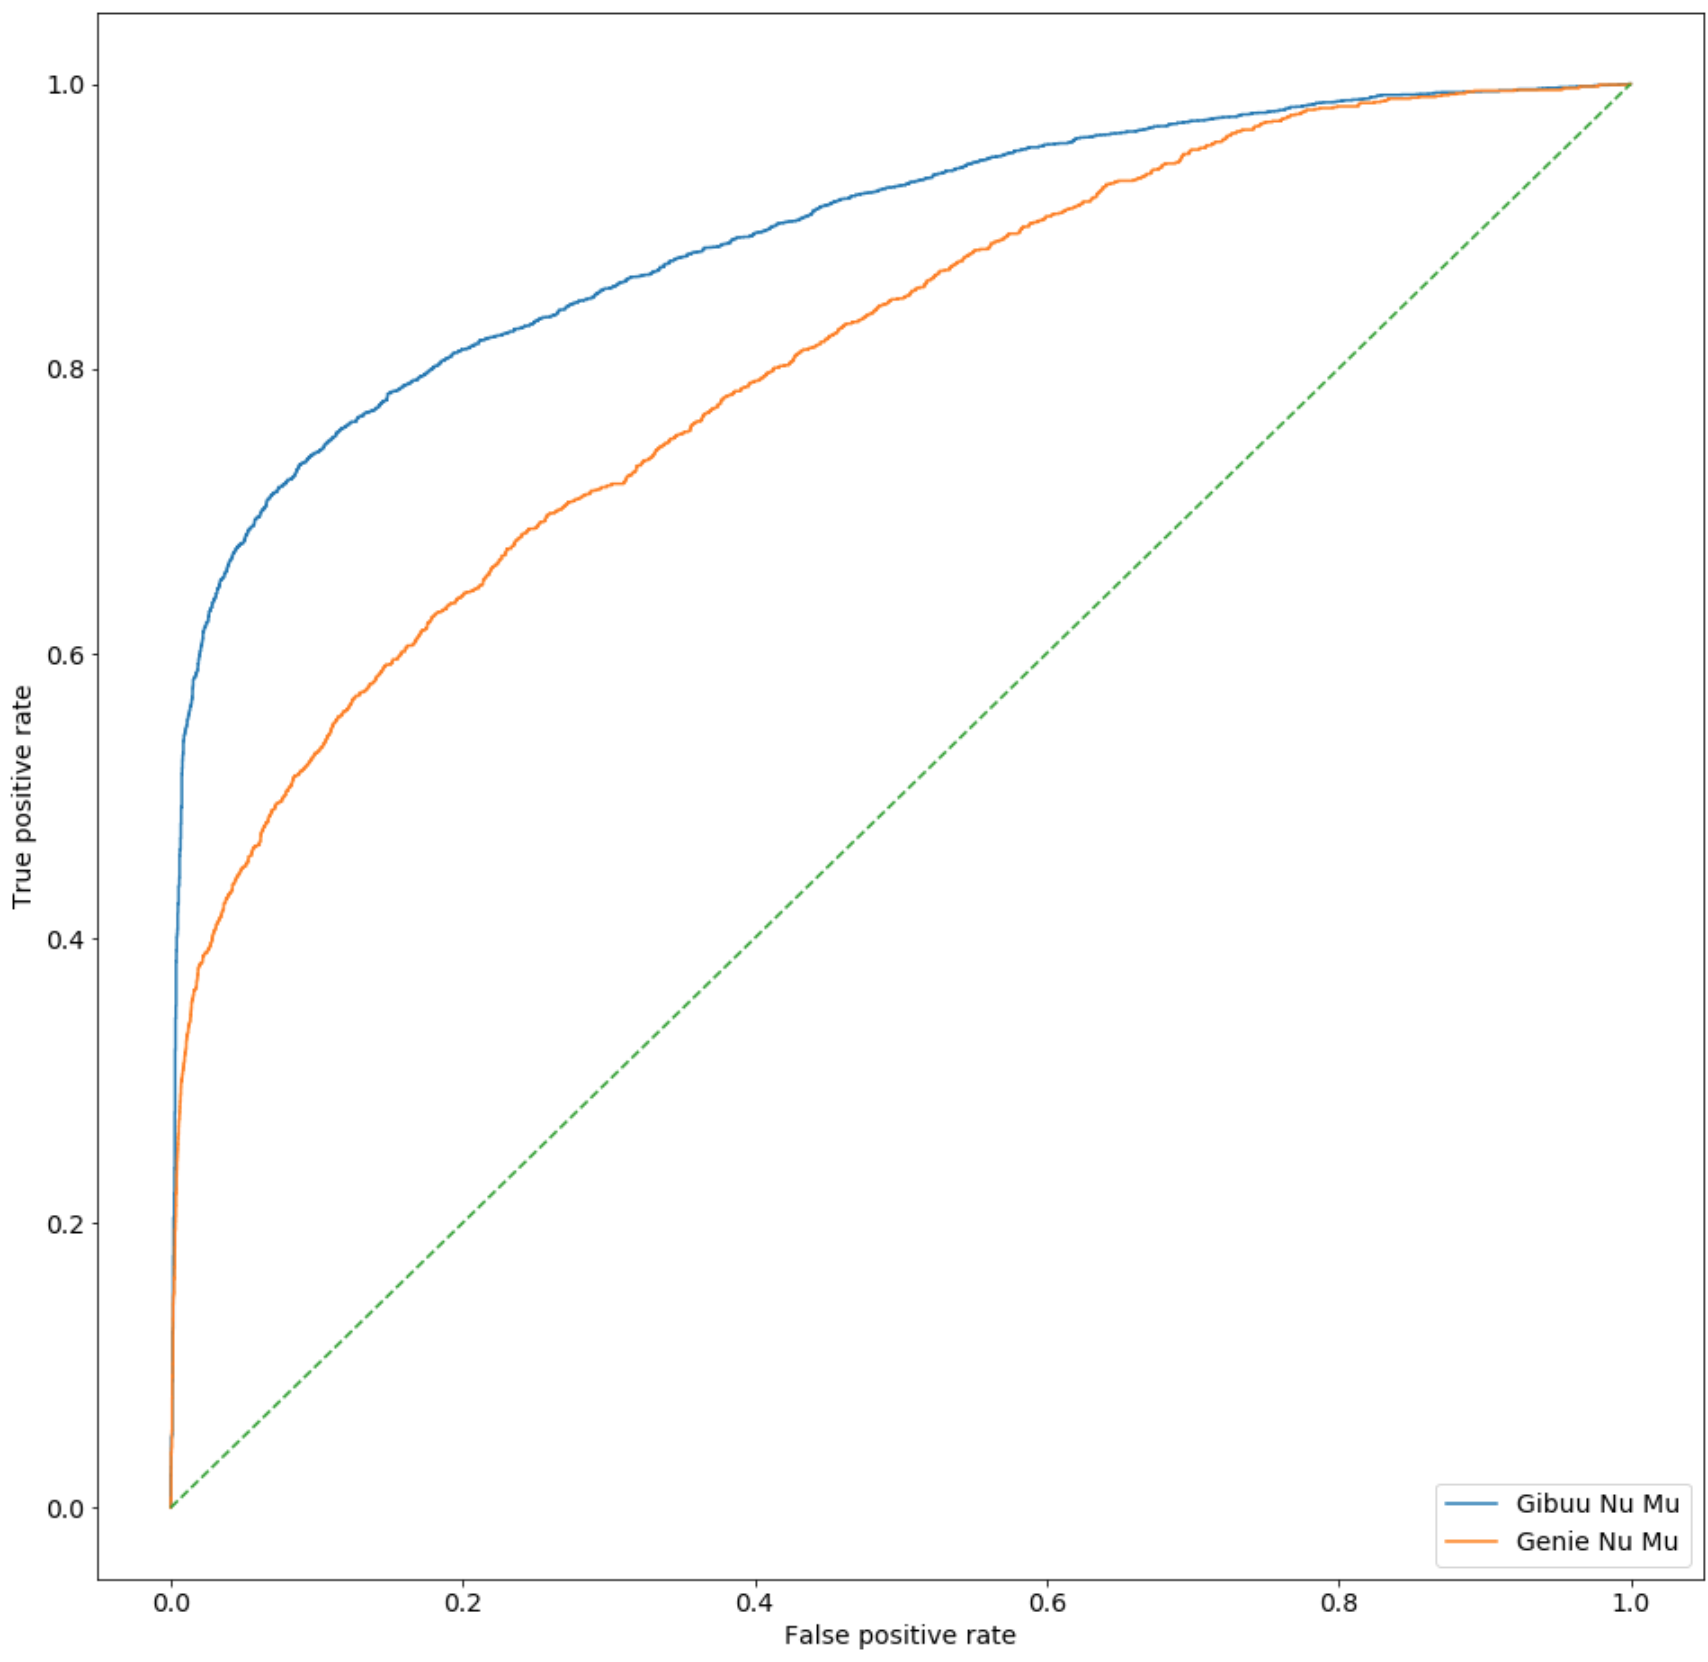
\includegraphics[width=75mm]{Both_Data/rocmu.png}
  \end{subfigure}
   \begin{subfigure}{}
 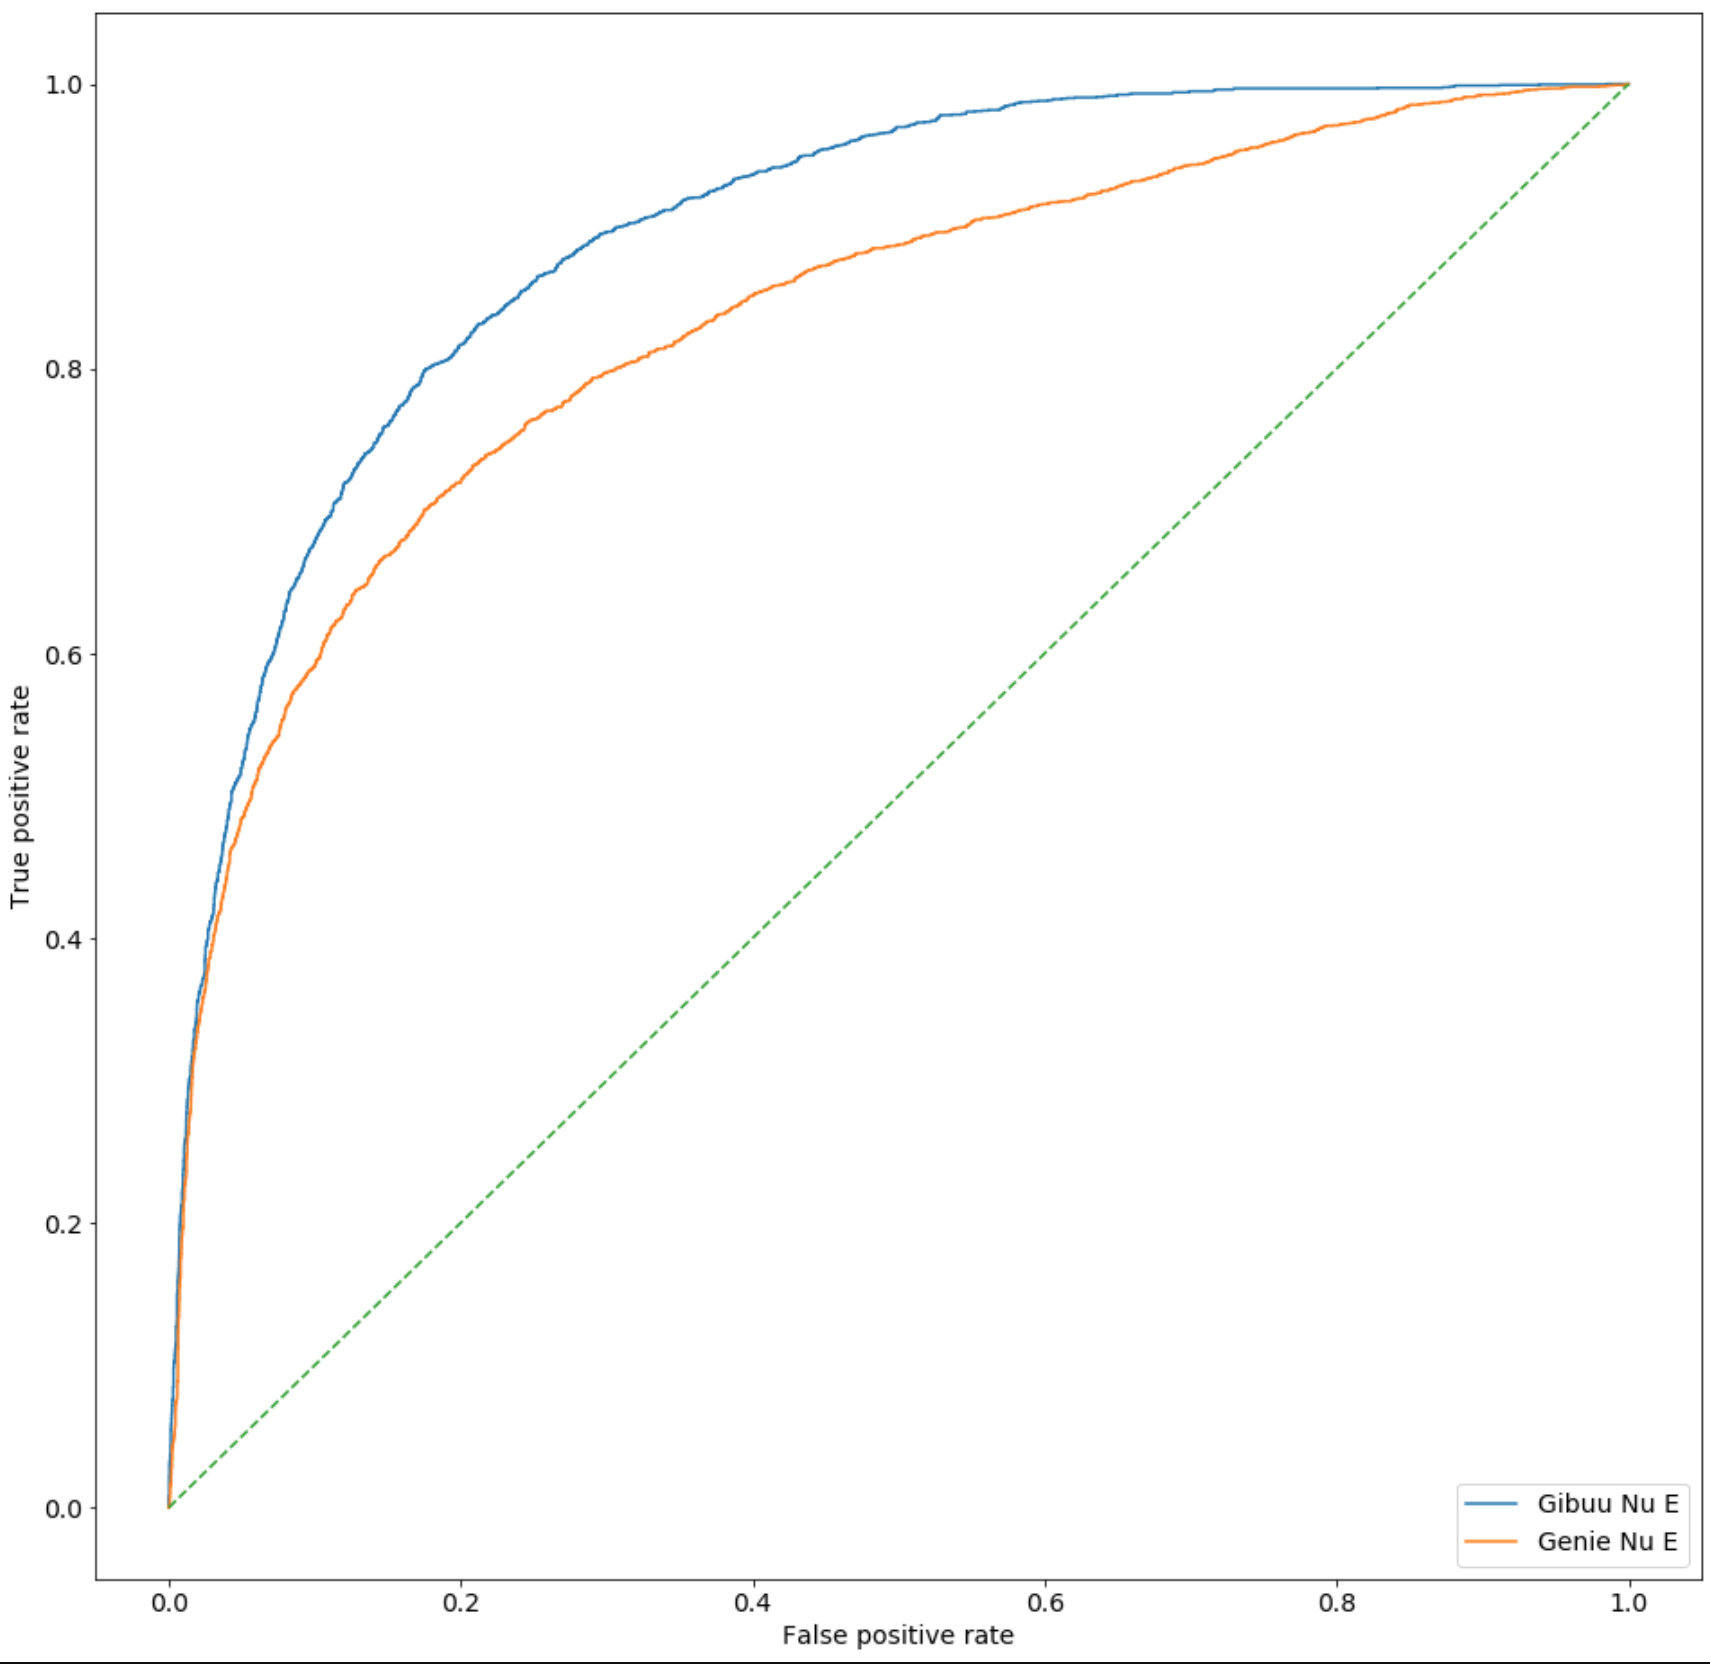
\includegraphics[width=75mm]{Both_Data/roce.png}
  \end{subfigure}
  
 \textbf{Figure 26.} \textit{ROC curves for $\nu_\mu$ classification on the left, and $\nu_e$ classification on the right. A blue curve represents GiBUU events and an orange curve, the GENIE events.}
\end{figure}

\noindent Using a Receiver Operating Characteristic (ROC) curve, which plots the true positive rate against the false positive rate of a binary classifier, in this case the classifier classifies whether the interaction was identified as a $\nu_\mu$ or not a $\nu_\mu$ event (and the same with the $\nu_e$ classifier to indicate how well the classifier performs, and provides a more intuitive visualisation for comparing performances. Figure 26 show the ROC curves for $\nu_\mu$ and the $\nu_e$ classifiers. The dotted line represents a random performance, and the closer a curve is to the upper left of the graph, the stronger the performance. By displaying the curves separately for GENIE and GiBUU events we are able to see that with both classifiers, the GiBUU events are classified with a higher accuracy than the GENIE events. This may be because a proportion of  GiBUU events are more distinctive in someway and the classifier learns how to classify these.\medskip







